\documentclass[12pt,a4paper,titlepage]{article}
\usepackage{graphicx}
\usepackage{amsmath}
\usepackage{amsthm}
%\usepackage{fullpage}
\usepackage{fancyheadings}
\usepackage{lastpage}
\usepackage{epsfig}
\usepackage{amsmath}
\usepackage{latexsym}
\usepackage{amssymb}
\usepackage{amstext}
\usepackage{fancyhdr}
\usepackage{array}
\usepackage{graphicx,picinpar,emlines2,epsf}

\setlength{\textwidth}{13.1cm}

\begin{document}
\setlength{\parindent}{0pt} \setlength{\parskip}{2ex plus 0.5ex
minus 0.2ex}

\title{Cardboard Comfortable When it Comes to Crashing}
\author{Team \# 24}
\date{April 16, 2003}

\maketitle

\fancyhead{} \pagestyle{fancy} \lhead{Team \# 24} \rhead{Page
\thepage\ of \pageref{LastPage}} \setlength{\headrulewidth}



\begin{abstract}


\noindent A scene in an upcoming action movie requires a stuntman
on a motorcycle to jump over an elephant.  Cardboard boxes will be
used to cushion his landing. To protect the nervous stuntman and
the motorcycle, we investigate various configurations of the
stunt.  We formulate a model for the energy required to crush a
box based on size, shape, and material.  We also summarize the
most readily available boxes on the market. We choose a maximum
safe deceleration rate of 5 g based on comparison with airbag rigs
used professionally for high fall stunts.  To ensure that the
stuntman lands on the box rig (rather than missing it completely)
we analyze the uncertainty in his trajectory and extract the
landing point uncertainty.  We go on to construct a numerical
simulation of the impact and motion through the boxes based on our
earlier box crush energy calculations.  After analyzing the
sensitivity and stability of this simulation, we use it to examine
the effectiveness of various configurations for the box stack
(including different box sizes, types of boxes, and stacking
patterns). Our findings indicate that 200 kg is the most desirable
combined mass of the motorcycle and stuntman. A 300 kg mass is
marginal and 400 kg is too heavy.  We also conclude that a launch
ramp angle of $20^\circ$ is optimal when considering safety,
camera angle, and clearance over the elephant. Our results show
that a stack constructed of (30 inch)$^3$ boxes with vertical
mattress walls spaced periodically is optimal when considering
construction time, cost, and cushioning capacity. We recommend
that this stack be constructed in dimensions 4 meters high, 4
meters wide, and 24 meters long. It will consist of approximately
1100 boxes and cost \$4300 in materials. The stuntman's wages are
uncertain but fortunately the elephant works for peanuts.


\end{abstract}


\tableofcontents
\newpage


\newpage

\begin{figure}
\centering
 \caption{\label{stunt} The death-defying leap over the
elephant!}
\includegraphics[width=0.8\textwidth]{whee.eps}
\end{figure}

\section{Introduction}

The American movie-going public's appetite for action and danger on the screen steadily
increases year by year.  The trend is clear: big budget + big action = big payoff.  Somewhere
in the darker alleys of Hollywood a desperate director decides to make a name for himself by
pulling off the biggest action sequence ever.  He plans to film a motorcycle jumping over the biggest
animal on land--the elephant!

Bureaucracy being what it is these days, Hollywood officials have hired us to ensure that neither
the stuntman nor the elephant is injured (of course, they could care less about the director).
The answer to keeping the elephant safe is simple: the elephant just stands in place and does nothing.
The safety of the stuntman is a more difficult problem.

Airbag rigs are commonly rented for high fall stunts \cite{MM}.  However, airbags
are designed only to catch humans.  Catching the motorcycle in the airbag would risk damaging it,
and replacement costs might well exceed the budget of our unnamed director.  The alternative
is to use a cardboard box rig--a stack of boxes that will crush and absorb the impact of the
motorcycle and stuntman.

{\bf We are now faced with the following:}
\begin{enumerate}
\item The primary objective is to safely catch the stuntman and motorcycle.
\item As a secondary objective, we wish to minimize the cost and size of the box rig.
\end{enumerate}

{\bf Our approach is:}
\begin{enumerate}

\item First we investigate the relationship between the size/shape/material of a box and the work required to
crush it.  We call this quantity the {\it crush energy} of a box.

\item We review the most commonly available cardboard box types.  We restrict our consideration to only
these types because custom boxes are much more expensive than standard ones.

\item By comparison with an airbag rig, we estimate the maximum acceptable deceleration that the stuntman
can experience during landing.

\item We analyze the trajectory of the motorcycle and the uncertainty in its landing location.  This determines the
proper placement of the box rig and how large an area it must cover to safely catch the motorcycle and stuntman.

\item Using the crush energy formula, we estimate the number of boxes that must be crushed in order to
arrest the motion of the motorcycle and stuntman.

\item We formulate a numerical simulation of the motorcycle as it enters the box rig.  Using this model we
analyze the effectiveness of various types of boxes and stacking arrangements.  We also compare low, medium,
and high trajectory jumps.

\item As an alternative to catching the stuntman while he is still sitting on the motorcycle, we analyze
the possibility of having the stuntman bail out in mid-air and land separately from the motorcycle.

\item Based on the results from our simulation, cost and construction considerations, and safety requirements,
we make a set of strong recommendations regarding placement, size, construction, and stacking type of the box rig.

\end{enumerate}


\section{The energy absorbed by crushing cardboard}

To calculate the ability of a cardboard box to absorb the impact of the stuntman and motorcycle we
estimate the energy required to crush the box.  This estimate is based on a combination of physical
considerations and experimental box crushing.

\begin{itemize}
\item  {\bf Assumption:} The primary source of energy absorption
is in the breakdown of the box walls due to edge compressive forces.
\end{itemize}

Commercial cardboard is rated by Edge Crush Test (ECT), which reports the pounds per inch of edge compressive force
parallel to the flute\footnote{The flute of corrugated cardboard is the wavy layer between the two wall
layers.  Here, {\it `parallel to the flute'} means the direction parallel to the flute wavefronts.}
which the cardboard can withstand before breaking.  This can be
interpreted as the force against the edge per unit length of crease created \cite{torhexpaper,4corrugated}.
Note that once a crease has formed, very little work is required to further bend the cardboard.

To understand how the formation of wall creases relates to the process of crushing a box, we conducted several
experiments by dropping a crush-test dummy on a box.  See Fig. \ref{fall} for illustration of experimental setup.

\begin{figure}
\caption{\label{fall} {\bf Experimental apparatus for crushing boxes.}  We dropped a crush-test dummy
(i.e. team member) onto several boxes and observed how the  structure broke down each time.}
\begin{center}
\includegraphics[width=0.4\textwidth]{fall4.eps}
\end{center}
\end{figure}

We observed that:
\begin{itemize}
\item The first wall-creases typically form in the first \%15 of the stroke distance.
\item These creases extend across two faces of the box (A schematic of one such crease is illustrated in Fig. \ref{creases}).
\item Once these have formed the box deforms further with comparatively little resistance because
 additional creases are created by torque forces rather than edge compressive forces.
\item The primary creases each have length approximately equal to the diagonal length of the face.
\end{itemize}
The work done in crushing the box is given by the average force applied times the distance through which it was applied.
This and the above experimental qualitative results lead us to write the following equation for energy absorbed by a box of dimension
$l_x \times l_y \times l_z$ being crushed in the z-direction.
\begin{equation}\label{crushenergy}
E = ECT \times \left(2\sqrt{l_x^2 +l_y^2}\right) \times l_z \times 0.15
\end{equation}

\begin{figure}
\caption{\label{creases} The first crease forms in a curve across the side faces as the box is compressed from above.}
\begin{center}
\includegraphics[width=0.25\textwidth]{crease.eps}
\end{center}
\end{figure}

{\bf As a reality check}, we compute the crush energy for a standard 8.5 in $\times$  17 in $\times$ 11 in box with ECT 20
lbs/in and C-flute (the type commonly used to store paper).  With these numerical values, Eq. \ref{crushenergy}
gives an energy of 187 Joules. This corresponds roughly to a 140 lbs person sitting on the box and nearly flattening it.
\begin{itemize}
\item {\bf Comparison with experiment:} Crush-test dummy results confirm that this is indeed a good estimate.
\end{itemize}

In addition to the crush energy, energy can also be absorbed in the process of flattening
the flute within the cardboard walls.  However, the pressure required to do this is
$\sim$150 kPa \cite{flutes} and the surface area involved is more than a square meter,
so a quick calculation show that the stuntman would decelerate too quickly if his kinetic
energy were to be transferred into flattening boxes.  We therefore ignore this additional flattening effect.
\begin{itemize}
\item Any successful box rig configuration must dissipate all of the kinetic energy of the stuntman and motorcycle through box crushing alone.
\end{itemize}

\section{Commonly available box types}

Minimization of costs is an important concern in this stunt.  The cardboard box rig will consist
of perhaps hundreds of boxes, and wholesale box prices can range up to \$10 or \$20 per unit (for larger
boxes), so we therefore restrict our attention to only those box types which are most commonly available.
We investigate the box types listed in table \ref{boxtypes}.

\begin{table}
\caption{\label{boxtypes} Commonly available box types. Information from \cite{papermart, veripack}.}
\begin{center}
\begin{tabular}{c |c | c | r} \\
Type &  Size (in) & ECT rating (lbs/in) & Price per box \\ \hline \hline
A & 10 $\times$ 10 $\times$ 10 & 32 & \$0.40 \\
B & 20 $\times$ 20 $\times$ 20 & 32 & \$1.50 \\
C & 20 $\times$ 20 $\times$ 20 & 48 & \$3.50 \\
D & 30 $\times$ 30 $\times$ 30 & 32 & \$5.00 \\
E & 44 $\times$ 12 $\times$ 12 & 32 & \$1.75 \\
F & 80 $\times$ 60 $\times$ 7  & 32 & \$10.00 \\
\end{tabular}
\end{center}
\end{table}

We will use this table later to evaluate the cost of various box rig configurations.

\section{Some quick estimates}

We now make a few rough calculations and estimates.  We will use these results to set safety
tolerances and as a guide in working with the more complex numerical simulation that we later formulate.

\subsection{Maximum safe acceleration}

To determine acceptable forces and accelerations for the stuntman as he enters the cardboard box rig,
we compare the box rig with other cushioning devices. In the stunt rigging business it is common practice to use an
air bag for high-falls of up to 30 meters.  Airbags rated for falls of up to 30 meters are approximately 4 meters deep.

Assume a stuntman falls from 30 meters above the airbag.  Gravity accelerates him from rest to a velocity $v$.  At this
point he strikes the airbag and is decelerated completely, so we have
$$
\sqrt{2 g d_{\scalebox{0.7}{\hbox{fall}}}}=\sqrt{2 a_{\scalebox{0.7}{\hbox{bag}}} h_{\scalebox{0.7}{\hbox{bag}}}}
$$
where $d_{\scalebox{0.7}{\hbox{fall}}}$ is the fall distance, $a_{\scalebox{0.7}{\hbox{bag}}}$ is the deceleration rate the
stuntman experiences in the airbag, $h_{\scalebox{0.7}{\hbox{bag}}}$ is the height of the airbag, and $g$ is the acceleration due to gravity. Thus
$$
a_{\scalebox{0.7}{\hbox{bag}}} = \frac{d_{\scalebox{0.7}{\hbox{fall}}}}{h_{\scalebox{0.7}{\hbox{bag}}}}g = \frac{30 \hbox{m}}{4 \hbox{m}}g = 7.5 g
$$
We therefore conclude:

\begin{itemize}
\item {\bf When using an airbag, the stuntman experiences an average acceleration of at most $7.5 g$}.  This
provides and upper bound on the maximum acceleration that a person can safely withstand.
\item {\bf However, with the airbag stunt the stuntman is able to land in a position that distributes forces evenly across his body.}  In our stunt
the stuntman will be landing in the box rig while still on the motorcycle.  This will result in greater chance for injury under high deceleration.
\item {\bf We choose $5 g$ as our maximum safe deceleration.} A box rig configuration which results in a higher acceleration will be rejected as unsafe.

\end{itemize}

\subsection{Displacement and energy estimates, a reality check}

If the deceleration of the stuntman and motorcycle is constant through the boxes then
we can estimate the distance required to bring him to rest.  Since any
deviation from constant acceleration will increase either the stopping distance or the
peak deceleration, this will give us a lower bound  on the stopping distance and hence a lower bound
on the required dimensions of the box rig.

Suppose the stuntman enters the rig at time $t=0$ with velocity $v_0$ and experiences a
constant deceleration $a$ until he is brought to rest at time $t=t_f$.  The stuntman's
velocity $v(t)$ is then given by $v(t) = v_0 - at$.  Since the stuntman is at rest at time $t_f$, we have
$$
t_f = v_0/a
$$
Let $x(t)$ be the displacement from the point of entry as a function of time.  Since $x(0) = 0$,
$$
x(t) = v_0t - (1/2)at^2
$$
and so the total distance traveled through the boxes is
$$
\Delta x = x(t_f) = \frac{v_0^2}{a} - \left(\frac{1}{2}\right)(a)\left(\frac{v_0}{a}\right)^2 = \frac{v_0^2}{2a}
$$
Therefore we arrive at:
\begin{itemize}
\item Given an impact velocity $v_0 \approx 20 m/s$ and deceleration bounded by 5 g, the stuntman will require {\it at least} 4 meters to come to rest.
\end{itemize}

Conversely, if we instead have an idea of what the stopping distance should be, we can easily compute
that the constant deceleration required to stop in a distance $\Delta x$ is $$ \frac{v_{0}^{2}}{2g\Delta x}.$$

Using the calculation for the energy dissipated by crushing a box we can estimate how many boxes must
be crushed to dissipate the energy of the incoming projectiles, i.e.: stuntman and motorcycle.
The energy that must be dissipated in the boxes is roughly equal to the kinetic energy that the
motorcycle and stuntman enter with.  (Since the box rig should only be three or four meters high,
the potential energy is a much smaller fraction of the total energy.)  Thus for $v_{0} = 20 m/s$
and a mass of 200 kilograms, the change in energy is 40,000 Joules.  From Eq. \ref{crushenergy} we
calculate that the crush energy of a standard (30 inch)$^3$ box is 633 Joules.
$$
\frac{40,000 \hbox{ Joules}}{633 \hbox{ Joules/box}} \approx 60 \hbox{ boxes}
$$
\begin{itemize}
\item {\bf Conclusion:} The incoming stuntman and motorcycle must crush about 60 boxes to come to a stop.
\end{itemize}

\section{Trajectory Analysis and Cushion Location}

Regardless of how much energy it takes to crush the cardboard boxes, they won't dissipate any of
the stuntman's energy unless he actually lands on them.  It is therefore important to consider
the trajectory of the stuntman and motorcycle through the air so we know where the box rig
should be placed and what the uncertainty in landing location is.

We calculate trajectories by solving the following  differential equation, where $v$ is
the speed, $k$ is the drag coefficient, and $\vec{x}$ is the position:
$$
(\vec{x})'' = -g\hat{z} - \frac{k}{m}|v|^{2}\hat{v}
$$
MATLAB's ODE45 function was used to solve an equivalent system of first order equations.  We use an air
drag coefficient of $k=1.0$ (this value is from Ref. \cite{drag}).  We see immediately from figure
\ref{correct_airres} that it would be unwise to ignore air resistance.
\begin{itemize}
\item {\bf Air drag effects alter the stuntman's landing position by up to several meters.}
We therefore incorporate air resistance into all simulations.
\end{itemize}

It is unreasonable to expect the stuntman to leave the ramp with exactly the same initial velocity and angle
every jump.  We therefore need to allow for some uncertainty in the resulting trajectory and ensure the
cardboard cushion is large enough to support a wider range of possible landing locations.  Since the ramp
angle $\phi$ is constant, we assume the initial angle between the direction of the stuntman and the ground
is also $\phi$ with no uncertainty.  However, there is the possibility that the motorcycle might be moving
slightly to the left or right as it leaves the ramp.   Let $\theta$ be the azimuthal angle between the ramp
axis and the stuntman's velocity vector.  Ideally $\theta$ should be zero, but small variations may occur.
The other uncertain initial condition is the initial velocity $v_{0}$.
\begin{itemize}
\item In modeling the stuntman's possible trajectories, we assume the following uncertainties:
\begin{itemize}
\item Initial velocity: $v_{0} = v_{\scalebox{0.7}{\hbox{intended}}} \pm 1$ m/s
\item Azimuthal angle: $\theta = 0 \pm 2$ degrees
\end{itemize}
\end{itemize}

We use this to identify the range of possible landing locations by plotting the trajectories
that result from the worst possible launches.  These are shown in Fig. \ref{uncer}.

If the intended initial velocity is 22 m/s, the ramp angle is $20^\circ$ and the mass of the rider
plus motorcycle is 200 kg, then
\begin{itemize}
\item {\bf Distance variation is:}  $\pm$ 2.5 meters.
\item {\bf Lateral variation is:} $\pm$ 1.5 meters.
\end{itemize}

\begin{figure}
\caption{\label{correct_airres}Air resistance significantly changes the trajectory.}
\begin{center}
\includegraphics[width=0.7\textwidth]{correct_airres.eps}
\end{center}

\caption{\label{uncer}Trajectory Uncertainty Due to Launch Uncertainties.  Note that the box rig depicted here is not to scale.}
\begin{center}
\includegraphics[width=0.7\textwidth]{uncer.eps}
\end{center}
\end{figure}

\section{Impact simulation}

In order to evaluate the effectiveness of various box rig configurations, we construct a numerical simulation
of the motion of the stuntman and motorcycle through the box rig.

\subsection{Assumptions}

The full physics of the box rig is far too complex to model accurately.  We therefore make the following
assumptions to approximate and simplify the problem:

\begin{itemize}

\item {\bf The problem is two dimensional.}  We restrict out attention to the plane of motion of the stuntman.
There is no reason for his trajectory to ever be significantly bent out of this plane.  Making this
simplification does remove the possibility of observing some box stacking effects.  However, we will
later show that these effects are negligible in most cases.

\item {\bf As the motorcycle plows through the boxes, a thick layer of crushed boxes accumulates against
its front and lower surfaces}.  These layers increase the effective size of the motorcycle and cause
it to strike a larger number of boxes as it moves.  We assume that this captures the effects of internal
friction and viscosity within the boxes.  A illustration of this effect is shown in Fig. \ref{debriswall}.

\item {\bf In the average of striking a large number of boxes, the velocity magnitude is reduced but the
direction is unchanged.}  A collision is as likely to deflect the trajectory upward as downward.

\item {\bf Boxes are crushed rather than pushed out of the way.}  In practice, this can be ensured by placing
a strong netting around the three sides of the box rig that face away from the incoming stuntman.

\item {\bf Boxes are crushed to a uniform level.}  In reality some boxes may be crushed only slightly,
while others are completely flattened, but these effects disappear when we average over a large number of box collisions.

\end{itemize}

\begin{figure}
\caption{\label{debriswall} A wall of debris forms on the front and bottom surfaces of the motorcycle as it enters the boxes.}
\begin{center}
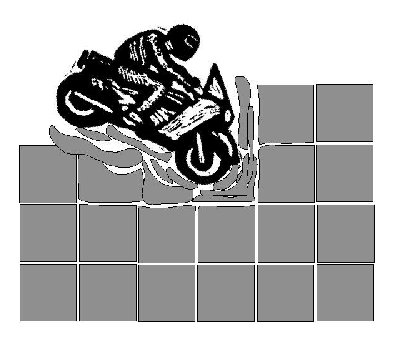
\includegraphics[width=0.4\textwidth]{crush2.eps}
\end{center}
\end{figure}



\subsection{Formulation}

We formulate the simulation as follows:

\begin{itemize}

\item The motorcycle and stuntman is represented by a bounding rectangle that is initially 1.2 meters long,
1.2 meters high, and 0.7 meters wide (though the width is irrelevant for most of the simulation).

\item The box rig is represented by a 2-dimensional stack of boxes.  We will consider several different
 stacking configurations.

\item We numerically integrate the motion in discrete time steps of 0.05 seconds.   The only object in motion
throughout the simulation is the stuntman and motorcycle--all of the boxes are stationary.

\item When the bounding rectangle intersects a box, the box is considered crushed.  We modify the stuntman's
velocity according to the kinematics described in the following section (see Eq. \ref{newvelocity}) and
ignore further interactions with the crushed box.

\item For each box crushed we add a layer of additional thickness to either the front or the bottom
(for horizontal and vertical collisions resp.) of the motorcycle bounding rectangle.  We assume
that boxes are crushed to \%20 of their length or height for horizontal and vertical collisions respectively.
We allow the front layer to extend above and below the original bounding rectangle (and likewise for the bottom layer)
so that the force of the motorcycle striking a tall box will effectively be distributed along the length of the box.
These debris layers increase the effective size of the motorcycle and therefore cause it to strike a larger
number of boxes as it moves.  We use this process to account for the effects of friction.

\item The vertical component of the velocity is set to zero when the bounding rectangle strikes the ground.

\end{itemize}

\subsection{Kinetics}

As the stunt person falls into the rig with the motorcycle each box he collides with will collapse and absorb
a small amount of his kinetic energy, thereby slowing his descent.

\begin{itemize}
\item Upon collision with a box, the box crushes
and absorbs an amount $\Delta E$ of energy from the stuntman's kinetic energy.
\item The crushed box is then pinned against the forward moving face of the stuntman and motorcycle and must move with him.
This contributes an additional mass of $m_{box}$.
\end{itemize}

We calculate the change in his velocity using conservation of energy and assuming that the
velocity direction remains unchanged (this is a good approximation in the average of a large number of collisions).
$$
\frac{1}{2}(m_0+m_{box})v_{new}^2 = max\left(\frac{1}{2}m_0 v_0^2 - \Delta E,0\right)
$$
and we are taking the maximum here to avoid imparting more energy into the box than the motorcycle has.
Solving for $v_{new}$ yields
\begin{equation}\label{newvelocity}
v_{new}=\sqrt{max\left(\frac{m_0 v_0^2 - 2\Delta E}{m_0 + m_{box}},0\right)}
\end{equation}
We use this equation to calculate the new velocity after each collision.

\subsection{Stability and sensitivity analysis}

Given the crude nature of our collision detection, there is the danger of finding results that depend sensitively
on the initial location of the motorcycle relative to the phase of the box rig periodicity (rig periodicity
is typically less than 1.5 meters).  To show that these phase alignment effects are negligible we vary the
initial location of the motorcycle by 0.4 meters (\%37 of the rig periodicity) either direction.

\medskip

{\bf Result:}  Deceleration rates and stopping distance vary by less than \%5.  The simulation is therefore
insensitive to where the motorcycle lands relative to the period of the box rig.

\medskip

As a second check, we vary the time step size from .025 to 0.1 seconds (0.05 is our standard value).

\medskip

{\bf Result:}  No distinguishable changes in results with variation in time step size.  This verifies
 that the simulation is highly insensitive to the size of the time steps.


\subsection{Configurations considered}

We consider the following configurations for the stunt:

\begin{itemize}

\item {\bf Three flight trajectories for the motorcycle and stuntman: low, medium, and high.}
These provide three different entry angles and velocities for the simulation.  Each trajectory is also
designed to clear an elephant that is roughly three meters tall \cite{elephant_facts}.  Details of these
trajectories are given in table \ref{trajectorytable} and they are shown to scale in Fig. \ref{trajectories}.

\item {\bf Seven different stacking arrangements.}  Details of these arrangements are shown in
Tab. \ref{stacktable} and Fig. \ref{stackfig}.

\item {\bf Three values for the total mass of the motorcycle and stuntman:} 200kg, 300kg, and 400kg.
These masses are reasonable for mid-range to large motorcycles.

\end{itemize}

\begin{table}
\caption{\label{stacktable} The seven box rig configurations that we examine.  See Fig. \ref{stackfig} for illustrations,
and refer to Tab. \ref{boxtypes} for box type data.}
\begin{center}
\begin{tabular}{c | c | c}
Stack type   & Cost                 & Comments \\
             &(per sq. meter)       &  \\ \hline \hline
1            & \$40.40              & Standard rig, made \\
             &                      & of box type $B$ (20in cube). \\ \hline
2            & \$94.20              & Standard rig, made of heavy duty \\
             &                      & box type $C$ (20in cube, ECT 48). \\ \hline
3            & \$43.10              & Standard rig, made of box \\
             &                      & type $D$ (30in cube).\\ \hline
4            & \$46.5               & Like 3, but type $A$ boxes \\
             &                      & placed inside the $D$ boxes.\\ \hline
5            & \$46.3               & Modification of 3--additional vertical \\
             &                      & walls of type $F$ mattress boxes.\\ \hline
6            & \$40.90              & Like 5, but horizontal mattress \\
             &                      & box walls.\\ \hline
7            & \$46.1               & Mattress boxes (type $F$) stacked \\
             &                      & horizontally, with periodic vertical walls\\
\end{tabular}
\end{center}

\caption{\label{trajectorytable} We simulate the stunt with the following three different trajectories.}
\begin{center}
\begin{tabular}{c | c | c | c}
Jump type   & Initial velocity     & Ramp angle  & Jump distance  \\ \hline \hline
Low         &    29 m/s            &  $10^\circ$ & 30.0 meters\\
Medium      &    22 m/s            &  $20^\circ$ & 28.5 meters\\
High        &    20 m/s            &  $30^\circ$ & 30.4 meters\\
\end{tabular}
\end{center}
\end{table}

\begin{figure}
\begin{center}
\caption{\label{stackfig} Box stacking configurations.  Crush patterns are the result of simulated impacts
of a 200 kg combined weight coming in from the low trajectory.}
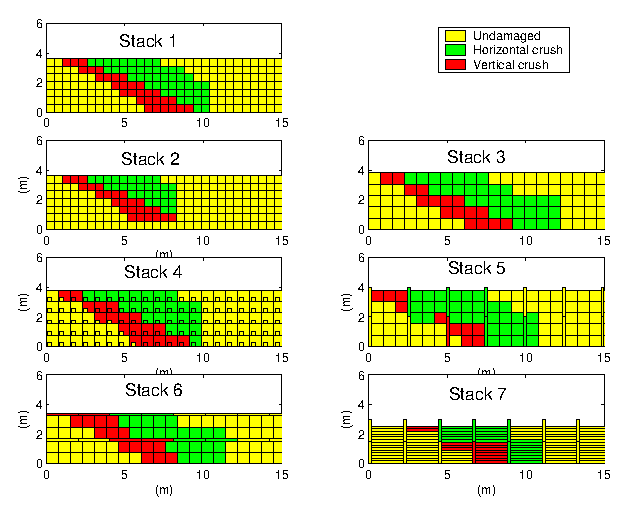
\includegraphics[width=0.65\textwidth]{stacktypes.eps}
\end{center}

\caption{\label{trajectories} The three trajectory profiles that we examine in our simulations.}
\begin{center}
\includegraphics[width=0.55\textwidth]{trajectories.eps}
\end{center}
\end{figure}

\subsection{Data analysis}

The simulation provides us with a record of the velocity as a function of time.  These velocity plots appear jagged
and step-like because of the discrete way in which our simulation handles collisions.  We obtain the acceleration by
fitting a straight line to the velocity vs. time plot and measuring the slope.  An example of this is shown in
Fig. \ref{velocityplot}.

\begin{figure}
\caption{\label{velocityplot} Velocity vs time; plotted for 200 kg low trajectory impact on box stack
type 1 (20 inch cubes, stacked in standard style).}
\begin{center}
\includegraphics[width=0.7\textwidth]{velocity_case_1_linear.eps}
\end{center}
\end{figure}

In examining the velocity plots for each simulation run, we looked at:
\begin{enumerate}
\item Deceleration experience by the stuntman, averaged over the {\it entire} time from impact to rest.
\item Maximum of deceleration averaged over 0.1 second intervals.
\item Whether or not the boxes completely arrested vertical motion before the stuntman hit the ground.
\end{enumerate}
If either (1) or (2) ever exceeds the maximum safe deceleration threshold of 5 g, we consider that configuration to be unsafe.
When condition (3) is not met then the stuntman may experience a severe and dangerous jolt as he strikes the ground.
This is bad, but we will propose some work arounds shortly.

\subsection{Results}

{\bf Regarding the mass}, 400 kg is too heavy--the boxes give way beneath the incoming motorcycle too easily.
It would require a stack of boxes nearly 6 meters high to safely catch this hot potato.  300 kg
is marginal, and 200 kg is optimal for using a box rig.

{\bf Stacking types}:
(refer to Fig. \ref{stackfig} for illustration)
\begin{enumerate}

\item Made from the cheapest and most common boxes, this stack resulted in 4.8 g deceleration,
which is within safety margins (but just barely).  It stopped the motorcycle in 11 meters$^\dagger$.

\item Rejected because is resulted in deceleration of over 6 g, but brings the motorcycle
to rest$^\dagger$ in only 7 meters.

\item Very soft deceleration of about 3.6 to 4.1 g.  The only problem is that this stack did not completely stop
 the vertical motion.  Also, it took 13 meters to bring the motorcycle to rest$^\dagger$.

\item Marginally safe deceleration from 4.8 to 5.1 g, but this stack is the best at arresting the
vertical motion.  Stopping distance of 9 meters$^\dagger$.

\item Behavior is similar to type (3), but stopping distance is reduced by 2 meters to 11$^\dagger$.

\item The extra horizontal mattress boxes make very little difference.  Deceleration is 4.1 g, and
vertical motion is not slowed enough to prevent hitting the ground hard.

\item Rejected because deceleration at 5.2 to 5.7 is considered unsafe.

\end{enumerate}
($\dagger$: Stopping distances are reported for the medium trajectory and are measured from the point of impact to the furthest box damaged.  The motorcycle actually comes to rest in a significantly shorter distance, but it pushes a wall of debris several meters ahead of it.)

\begin{itemize}
\item {\bf Hypothesis:} the difficulty of slowing the vertical motion enough might be overcome by stacking
the box rig on top of a landing ramp.
\item {\bf Conclusion:} These results indicate that type (1) stacking is optimal without a ramp.  However,
with a landing ramp under the boxes, type (3) or type (5) stacking may be used to achieve a much softer deceleration.
\end{itemize}

In light of these results, we tried additional variations on the type (5) stack.  We conclude that
the 30 inch boxes (type $D$) with mattress box walls spaced every 4 boxes is optimal.


\section{An alternative idea: the stuntman could bail out mid-flight}
So far our goal in this model has been to safely decelerate the total combined mass of the stuntman and his
motorcycle.  However, it is possible that they may separate before impacting the box rig.  In fact, it may even be desirable
for this separation to occur because it would reduce the chance of injury resulting from the
stuntman being pinned against the motorcycle.  We would therefore like to model how far apart the stunt person and the
motorcycle could land.  We assume they separate after clearing the elephant and allowing for a clear camera shot.  This
corresponds to a distance of about 25 meters.  We then run the same simulation as before but alter the vertical velocity
at the point of separation and then follow separately the two different trajectories.  An estimate of the change of momentum is
necessary to figure out the corresponding changes in velocity.  If the stuntman jumps vertically away from the motorcycle, it
makes sense to consider the analogy of a person jumping on the ground.  A decent jump corresponds to about half a meter.  Since
the initial velocity is given by $v_{0} = \sqrt{2gd}$ where $d$ is the height, we find that $v_{0}$ is roughly 3 m/s.  Accordingly,
we increase the stuntman's vertical velocity by 3 m/s.  Then the corresponding change in velocity for the motorcycle is given
by conservation of momentum.  The resulting trajectories are plotted in figure \ref{separation}.

\begin{figure}
\caption{\label{separation}stuntman separating from motorcycle in three possible trajectories.}
\begin{center}
\includegraphics[width=0.7\textwidth]{separation.eps}
\end{center}
\end{figure}

When the trajectory is medium or high, stuntman and motorcycle are only separated by about six meters at the point of landing in the cardboard boxes.
When the trajectory is low, however, this separation increases to around 15 meters.  This presents a problem if we want to protect both the
motorcycle and the stuntman.  Naturally, the safety of the person is the most important.  It is simple to extend the box rig to the projected
landing location of the stuntman.  Unfortunately, simulations show that a box configuration designed to smoothly decelerate the combined mass
of motorcycle and stuntman doesn't work as well when there is just the mass of the person to contend with.  In fact, it's possible
that the stuntman will decelerate so quickly that our g-force tolerance is exceeded.  Our simulations show that this is in fact the case for {\it all} of the box stacks that we considered.  For the heights and speeds considered, a box rig is unsafe.  %added
However, if the boxes are stacked loosely enough with some spacing between the boxes as in figure \ref{personcrash}, then it is still possible to
decelerate the stuntman at a reasonable rate.

Therefore the best solution for the safety of the stuntman is to re-design the box rig, using a softer material and/or looser stacking, so that it
accounts for his mass alone if he does indeed intend to separate from the motorcycle.

\begin{figure}
\caption{\label{personcrash} Box stacking arrangement that is suitable for catching a stuntman who is {\it not} on a motorcycle.}
\begin{center}
\scalebox{1.0}[0.8]{\includegraphics[width=0.7\textwidth]{person_crash.eps}}
\end{center}

\end{figure}


\section{Recommendations}

\begin{itemize}

\item {\bf Which mass is best?}  Our simulations show that a 400 kg mass is simply too heavy to be
adequately slowed by a box stack less than 4 meters high.  The motorcycle invariably falls
through the rig and hits the ground beneath at over 5 m/s.  While this may not seem like much,
the motorcycle could easily tumble over in the boxes and crush the stuntman along with the cardboard.
The 300 kg mass was marginal, but the safest was 200 kg. Therefore, if there is any choice in
filming the scene, we strongly recommend the use of a lighter motorcycle.

\item {\bf Which trajectory is best?}  The low trajectory ($10^\circ$) provides the least risk of coming
down too hard.  However, it allows only minimal clearance over the elephant (only 1 meter for a tall elephant)
and requires the highest speed to make the jump successfully, which increases the risk.

\item {\bf Which type of boxes and stacking is best?}  The type (1) stack, made of (20 inch)$^3$
boxes, is best for landing without a ramp.  With a ramp under the
rig, type (3), made from (30 inch)$^3$ boxes, and type (5), which
is type (3) with added vertical mattress box walls, are optimal.
The added walls of type (5) decreased the landing distance by 2
meters, so fewer boxes are required and the construction cost is
reduced.

\item {\bf What size must the rig be?}  With the 200 kg mass our simulation shows that 3 meters height are usually
enough for the low trajectory, but 4 are necessary for the high trajectory.  This can be reduced to as
little as 2 if the rig is stacked on top of a landing ramp.  Stopping distance is between 10 and 13 meters
(as measured from point of entry to the front of the debris wall) depending
on stack type, and we estimate in \S6 from the trajectory variability calculation that the landing location
uncertainty is 1 meter laterally and 3 meters forwards or backwards.  We consider an additional $\%50$ beyond these uncertainties
to be necessary to suitably ensure safety.  Therefore our recommendations are:
\begin{itemize}
\item Height should be 4 meters without landing ramp, 2 meters with ramp.
\item Width should be 4 meters.
\item Length should 24 meters for type (1) or (5) stacking, and 29 meters for type (3) stacking.
\end{itemize}

\item {\bf How much does it cost?}  The cost is between \$4300 for type (1) and \$5300, depending
on the precise configuration.  Note that this is approximately the same as the cost of renting an
airbag rig for a day \cite{MM}.

\item {\bf How many boxes is that?}  Type (1) stack requires 2000 (20 inch)$^3$ boxes, and type (3) requires 1100 (30 inch)$^3$ boxes.
Type (5) uses the same number as (3) and a few additional mattress boxes.

\end{itemize}

{\bf Final recommendation:} The overall best type of box rig to use is (5)--(30 inch)$^3$ boxes stacked as usual,
with vertical mattress box walls every couple meters to distribute the forces over a larger number of boxes.  This
configuration results is the softest deceleration while still effectively stopping the stuntman and motorcycle.  It
also requires the fewest boxes, so the cost is lower and the setup time is minimized.  This configuration is shown in detail in Fig. \ref{case7}
\begin{figure}
\caption{\label{case7} The best way to stack the boxes.}
\begin{center}
\scalebox{1.0}[0.8]{\includegraphics[width=0.7\textwidth]{case73.eps}}
\end{center}
\end{figure}

\newpage
\begin{thebibliography}{99}
\bibitem{MM}{www.mmstunts.com, Accessed Feb. 7th, 2003.}
\bibitem{torhexpaper}{torhexpaper, Accessed Feb. 7th, 2003.}
\bibitem{veripack}{www.veripack.com, Accessed Feb. 7th, 2003.}
\bibitem{papermart}{www.papermart.com, Accessed Feb. 7th, 2003.}
\bibitem{4corrugated}{www.4corrugated.com, Accessed Feb. 8th, 2003.}
\bibitem{drag}{http://aerodyn.org/Drag/tables.html\#man, Accessed Feb. 8th, 2003.}
\bibitem{elephant_facts}{http://www.zoo.org/chai/site/learn/african.htm, Accessed Feb. 8th, 2003.}
\bibitem{boxpicture}{http://www.affordable-removals.co.uk/stacked\_boxes.gif, Accessed Feb. 8th, 2003.}
\bibitem{cardboard density}{http://www.cam.ac.uk/societies/cuecs/addenbrook/addenbrook.html, Accessed Feb. 8th, 2003.}
\bibitem{flutes}{Jochen Pflug, Ignaas Verpoest and Dirk Vandepitte, {\it Folded Honeycomb Cardboard and Cpre Material for Structural Applications}  http://www.mtm.kuleuven.ac.be/Research/C2/poly/downloads/SC5\_TorHex\_Paper.pdf, Accessed Feb. 7th, 2003.}
\bibitem{motopic}{http://www.journeywoman.com/traveltales/chinese\_english\_teacher.html, Accessed Feb. 9th, 2003.}
\bibitem{boxterminology}{http://www.scapackaging.com/doc/Corrugated\_Glossary\_-\_explanation.pdf, Accessed Feb. 7th, 2003.}
\bibitem{elephant_pic}{http://www.vegsoc.org/vegginout/images/elephant.gif, Accessed Feb. 8th, 2003.}
\bibitem{boxdensity}{http://www.tis-gdv.de/tis\_e/verpack/papier/begriffe/begriffe.htm, Accessed Feb. 8th, 2003.}
\bibitem{ECT}{http://www.tharco.com/packinginfo/environmental/alternativerule.html, Accessed Feb. 7th, 2003.}


\end{thebibliography}

\end{document}
%w00t
